\section{Proposed Software Architecture}
\subsection{Subsystem Decomposition}
\begin{figure}[H]
	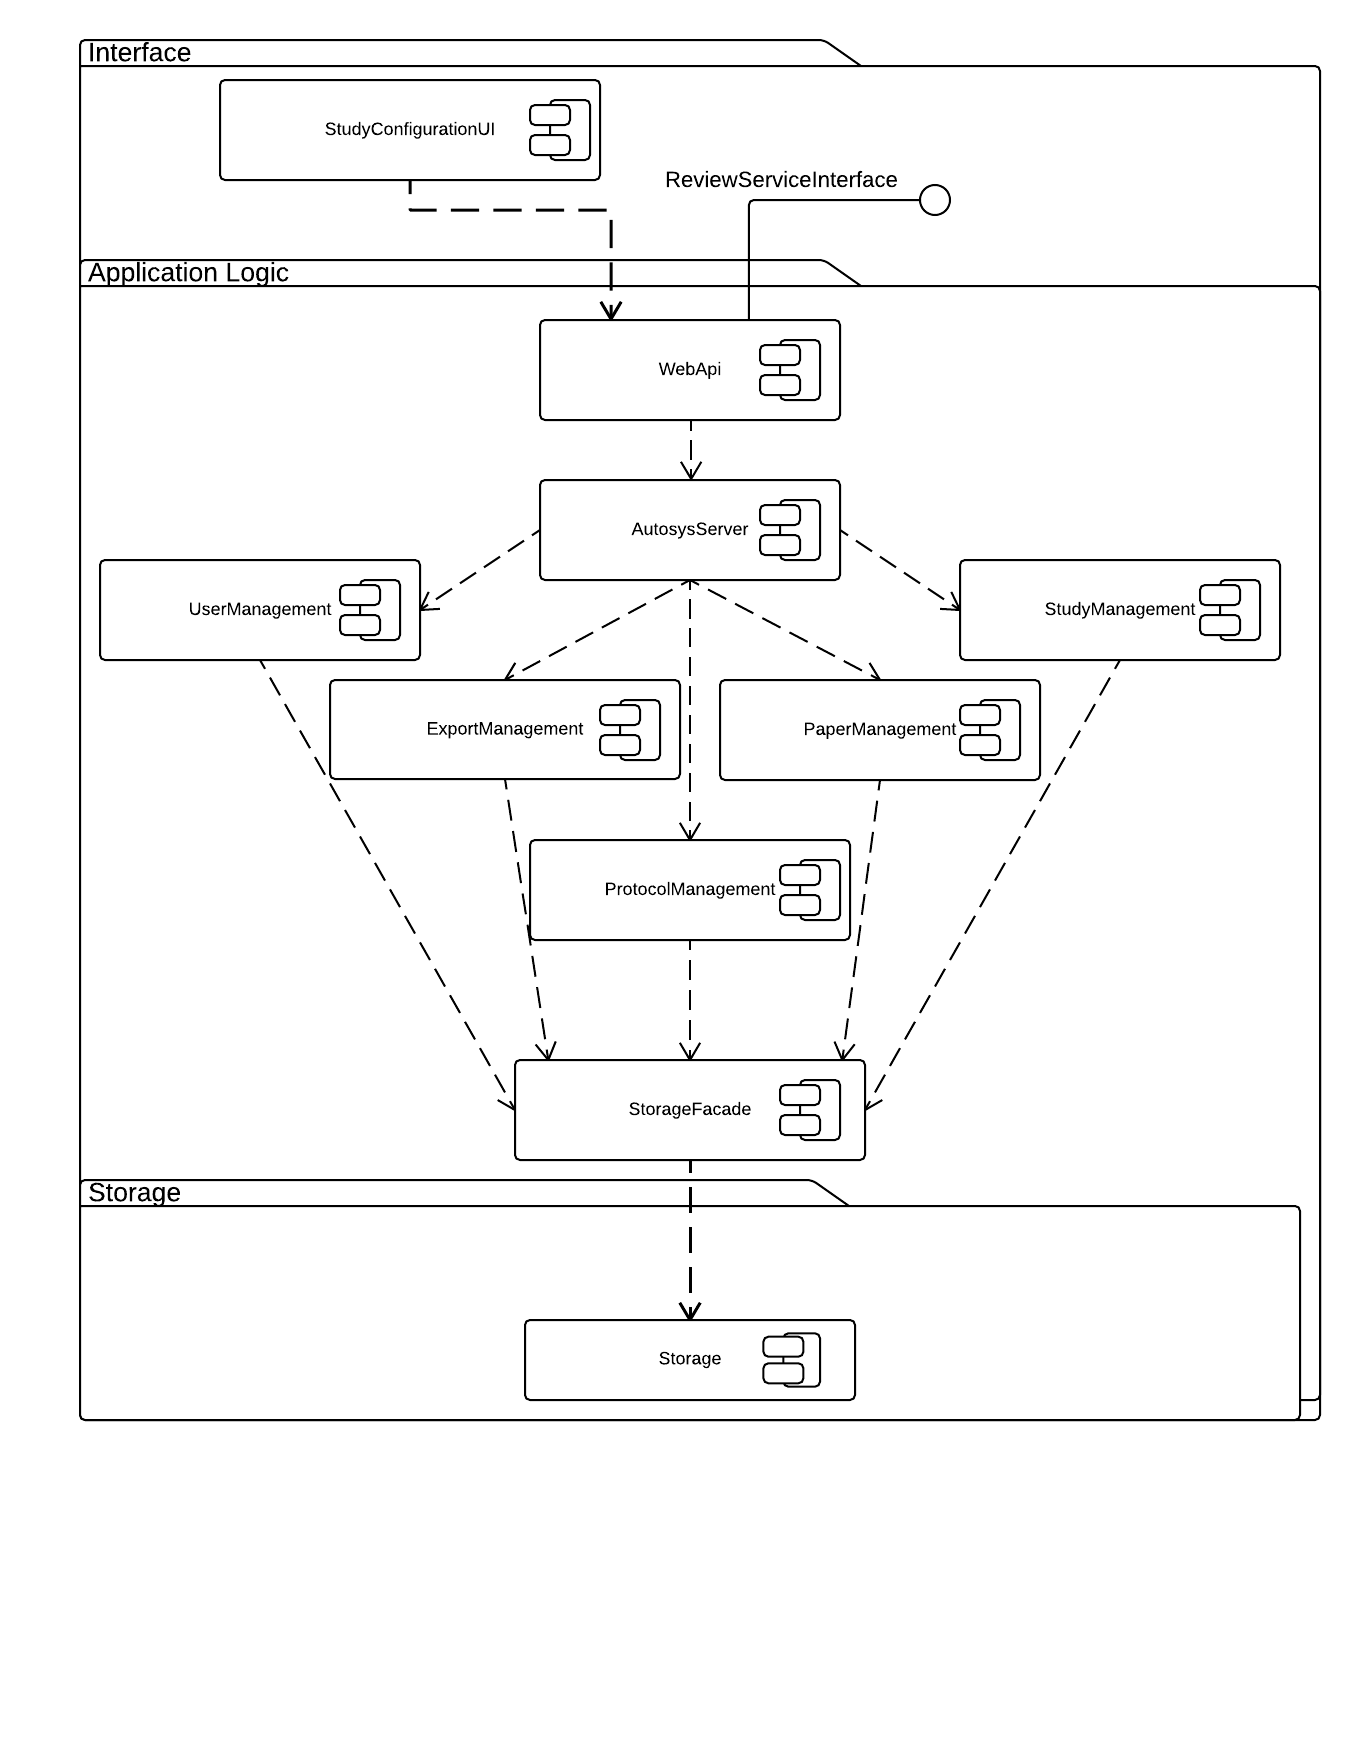
\includegraphics[width = \linewidth]{UMLComponentDiagramSubsystems}
	\caption{Autosys subsystem decomposition (UML Component Diagram, layers shown as UML packages)}
	\label{fig:Subsystem Decomposition, UML Component Diagram}
\end{figure}
The subsystems are identified from the functional requirements of the Autosys RAD document. A three-tier architectural style has been used for the decomposition of the system where a \textbf{StudyConfigurationClient} provides a front end for users to initiate all use cases related to setting up or configuring a \textbf{Study}. Also a \textbf{StudyReviewClient} will provide the front end for users to manage teams, and work with review tasks.
The \textbf{AutosysServer} will be managing access control, concurrency control, and delegates to nested subsystems for the application logic. The \textbf{UserManagement} component is holding the responsibility for handling all CRUD operations regarding teams and individual users. The processing of all Study related CRUD operations are carried out by the \textbf{StudyManagement} component. The  \textbf{StudyManagement} also manages Study Tasks, Study Criteria and Classifications, Study Phases and he other parts included in a study. The \textbf{PaperManagement} runs the filtering mechanisms on the research papers and does import/export of research papers according to the Study Criteria and Classifications.
The\textbf{ IStorage} interface is used for a Bridge Pattern to decouple the storage abstraction from the application logic so that the two can vary independently. At the bottom tier the \textbf{AutosysStorage} represents the subsystem for storing the user data, study data, and research papers.

\subsection{Identifying and Storing Persistent Data}
\paragraph{Identifying persistent objects}\mbox{}\\
Autosys deals with three sets of objects that must be stored.  The first set consists of research data that are accessed during conduction of secondary studies. The second set consists of objects that are created and accessed by the blue part of the system(eg. Users, roles, tasks). It need to be persistent to track the progress of the study, who is involved. The third set consists of data for a study configuration that are created by the study configuration UI.\\\\ The first set of objects is well defined and will rarely change during the lifetime of Autosys. These changes may occur whenever new research data has been created or removed and thus create a need for an update of the set. The second set of objects are managed and defined by the blue part of the system. Hence, we decide to let the blue part decide how to manage and access these persistent object through a generic interface. The third set of objects is also well defined and will not change once the study configuration has been made.

In this scope of the Autosys system, the main focus are set on the first and third set of persistent objects.  

\paragraph{Selecting a storage strategy}\mbox{}\\
By selecting and defining a persistent storage strategy enables us to deal with issues related to storage management. The main design goals of the yellow part of Autosys are to be reliable, scalable while also have high performance. It is therefore decided to implement a database management system because it allows concurrent queries and provide transaction mechanisms to ensure data integrity. \\\\Compared to a flat file storage method, a database management system will also scale to large installations with many researchers that are to conduct studies simultaneously. However, to allow future upgrades or changes it has been decided that the storage strategy is not solely dependent on a database management system. Thus, the Istorage subsystem will provide an abstract interface that enables other kinds of storage to be coupled. The users of Autosys are not able to change the storage, however if an update is ever needed for the storage strategy, a system administrator are able to do so.    

\subsection{Hardware/Software mapping}
\paragraph{Systems}\mbox{}\\
This program is inherently a documentation tool which map research articles goals and conclusions in a searchable context. This requires the program to be stable and reliable, especially  in the context of data preservation. \\The program is split in two components, a client and a external database  server. The user will run a client on his computer which will communicate with the server which runs the application logic and storage. The user client will feature data preservation, to enable offline functionality, but only to a limited extend. This report primarily focus on the server, if any questions to the user client should occur,  please refer to the according Blue SDD.\\ \\
All user clients will contact the a single server. To solve this, the server will be multi threaded, which allows for multiple users interacting with the server at the same time, but  At the current scope of the program, this is possible due to low amount of users, but should this system expand a new design should be conceived. \\
\begin{figure}[H]
	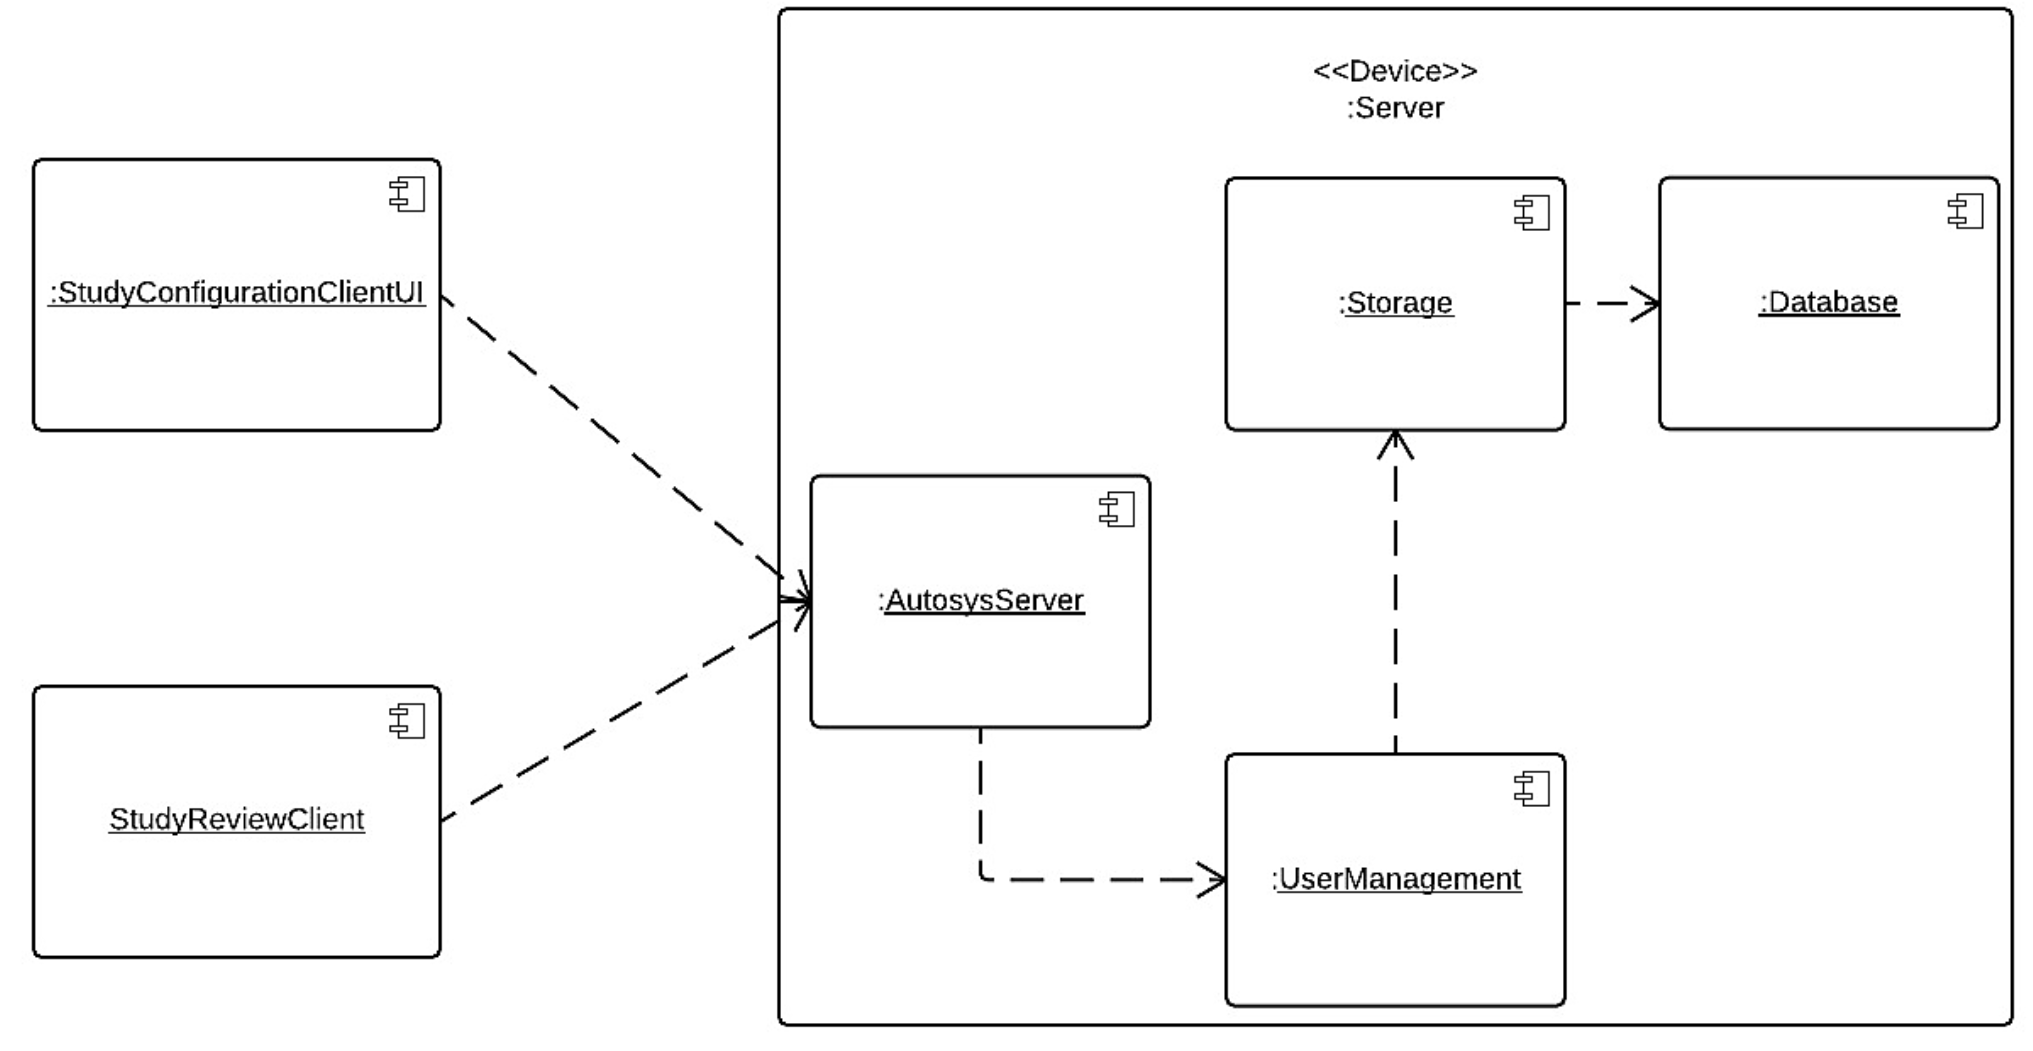
\includegraphics[width=\textwidth]{mappingImage}
\end{figure}
\paragraph{Program components}\mbox{}\\
The server will be implemented in C Sharp as requested by the the client. By using C Sharp, we can utilise to Microsoft expansive database systems and interfaces especially in regards to the database. Additionally this also make the program easier to maintain, since C Sharp is a well known language and can utilise the .NET framework. As communication between the server and the clients, we plan to communicate with HTTPS  request containing JSON object. This will make it easier to implement future changes and even completely replace the clients user interface with a more modern solution like a web page